\documentclass{jsarticle}
\usepackage{otf}
% パッケージの読み込み
\usepackage[dvipdfmx]{graphicx}
%
%\defaultfontfeatures{Mapping=tex-text}
%\setromanfont[Mapping=tex-text]{Hoefler Text}
%\setsansfont[Scale=MatchLowercase,Mapping=tex-text]{Gill Sans}
%\setmonofont[Scale=MatchLowercase]{Andale Mono}
\begin{document}
\begin{center}
 \textgt{{\LARGE コンピュータビジョン  自由制作課題説明書}}
\vspace{30mm}
\end{center}
% 図の挿入
\begin{figure}[htbp]
\begin{center}
\includegraphics[width=66mm,height =45mm]{copy.jpg}   
\includegraphics[width=66mm,height=45mm]{aurora1-1.jpg}
\\   
\includegraphics[width=66mm]{aurora1-2.jpg}   
\includegraphics[width=66mm]{aurora1-3.jpg}

\end{center}
\end{figure}

\newpage
% 目次の表示
\tableofcontents
\newpage
% 本文
\section{ 作品1について}
\begin{figure}[htbp]
\begin{center}
\includegraphics[width=100mm]{copy.jpg}  
\end{center}
\end{figure}

\subsection{制作作品コンセプト}
この画像のテーマはハワイです。日の入りの海面で踊るフラダンサー達が水面に反射しているのを表した、ファンタジーな作品です。落ちていく太陽の光によってシルエットになっているダンサーをイメージしました。\\
\hspace{3mm}今回のコンセプトが壁紙画像だったので、PCで作業後の疲れ目に、まるで遠くを見ているかのような画像を壁紙に設定することで、視力の回復を見込みたいと考えました。また、水面の模様と影に透過処理を用いて、水面に映る画像処理に挑戦してみたかったことと、私自身がハワイに行きたいという願望から、このテーマに決めました。
\subsection{使用したクラスについて}
作品1に用いたクラスと、その目的を記します。
\\
\underline{・Binalization.java}\\
シルエットが欲しかったので、画像を白と黒の2値のみにするために用いた。
元の画像はシルエットの画像だが、背景や境界線に白黒以外の色も混じっているので、この作業は必要である。
\\
\\
\underline{・Scale.java}\\
シルエット画像の大きさの調整を行なった。
\\
\\
\underline{・Rotation.java}\\
水面に映る影を作るためにまずは180度回転の幾何変換を施すために使った。
\\
\\
\underline{・Kmeans.java}\\
Chromakey処理に使うために、画像を領域分割させて減色させた。今回は引数に6を指定したので、6色に減色されている。
\\
\\
\underline{・Chromakey.java}\\
先に述べたKmeansクラスを用いて、背景からシルエットの部分のみを抜き出す処理を行うために用いた。
\\
\\
\underline{・AlphaBlending(画像に依存した投資番号).java}\\
合成するフラダンサーのシルエット画像によって固有のAlphaBlendingのクラスを作成した。\\
倒立していないフラダンサーの画像に関しては、合成位置指定と透過処理のために用いた。\\背景の地平線の画像の上に4枚の画像がバランスよく並ぶように位置を指定して合成した。\\
透過処理では、水面の波の模様とダンサーの画像が混じるように処理を施した。\\
それに対して、倒立している反射面の方のフラダンサーの画像のために、上記のような合成位置指定と透過処理の目的に加えて、180度幾何変換させた画像をさらに、左右反転させる処理を施した。\\
左右反転の処理では、x軸方向の出力を操作して実現することができた。\\
\subsection{用いた画像}
\begin{figure}[htbp]
\begin{center}
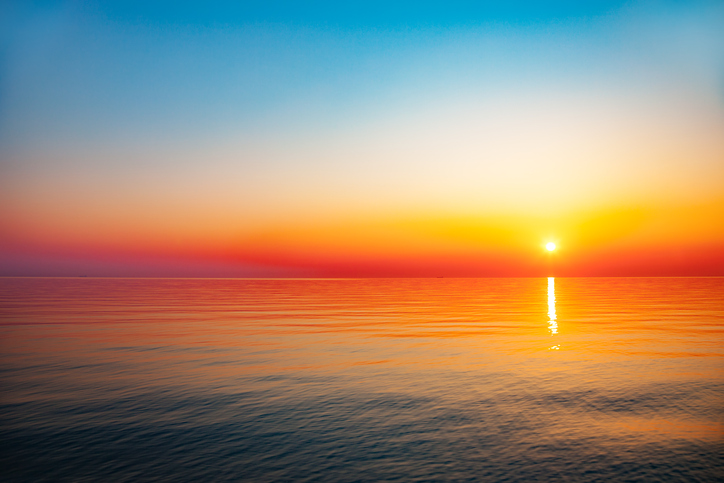
\includegraphics[width=52mm]{sunset.jpg}  
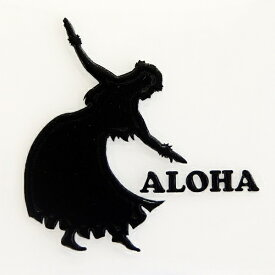
\includegraphics[width=35mm]{hawaii2.jpg}  \\

\includegraphics[width=30mm]{hawaii3.png}  
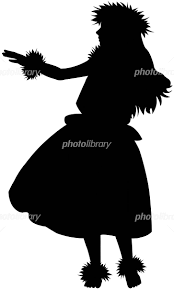
\includegraphics[width=26mm]{hawaii4.png}  

\includegraphics[width=30mm]{hawaii5.png}  
\end{center}
\end{figure}

\subsection{使用手順}
以下に適用したクラスとその効果をピックアップしたものです。\\
%\begin{figure}[htbp]
%\includegraphics[width=50mm,height =35mm]{image1.jpg}  
%\caption{} 
%\includegraphics[width=50mm,height =35mm]{image2.jpg}  
%\caption{}
%\end{figure}
\begin{figure}[h]
    \begin{tabular}{cc}
      %---- 最初の図 ---------------------------
      \begin{minipage}[t]{0.45\hsize}
        \centering
        \includegraphics[keepaspectratio, scale=0.3]{image1.jpg}
        \caption{}
    %    \label{ラベル1}
      \end{minipage} &
      \hspace{3mm}
      %---- 2番目の図 --------------------------
      \begin{minipage}[t]{0.45\hsize}
        \centering
        \includegraphics[keepaspectratio, scale=0.3]{image2.jpg}
        \caption{}
      %  \label{ラベル2}
      \end{minipage}
      %---- 図はここまで ----------------------
    \end{tabular}
  \end{figure}
  \\
図1は、hawaii2.jpgにScale.javaを用いて大きさの調整、AlphaBlending.javaを用いて合成位置の調整をしてsunset.jpgに合成をしたものである。\\
図2は、図1のhawaii2.jpgの背景が邪魔なのでBinalization.javaで背景を切り取ったものである。
\begin{figure}[h]
    \begin{tabular}{cc}
      %---- 最初の図 ---------------------------
      \begin{minipage}[t]{0.45\hsize}
        \centering
        \includegraphics[keepaspectratio, scale=0.3]{image3.jpg}
        \caption{}
    %    \label{ラベル1}
      \end{minipage} &
      \hspace{3mm}
      %---- 2番目の図 --------------------------
      \begin{minipage}[t]{0.45\hsize}
        \centering
        \includegraphics[keepaspectratio, scale=0.3]{copy.jpg}
        \caption{}
      %  \label{ラベル2}
      \end{minipage}
      %---- 図はここまで ----------------------
    \end{tabular}
  \end{figure}
  \\
  図3は、図2のようにAlphaBlendingクラスを用いて、合成位置と透過処理を施して、複数のシルエット画像をバランスよく並べたものである。
  図4は、180度回転・反転させて複数をちょうど影になるような位置に配置したものである。
\newpage
\section{作品2について}
\begin{figure}[htbp]
\begin{center}
\includegraphics[width=50mm]{aurora1-2.jpg}  
\includegraphics[width=50mm]{aurora1-3.jpg}  
\includegraphics[width=50mm]{aurora1-1.jpg}  
\end{center}
\end{figure}
\subsection{制作作品コンセプト}
この作品は、元の画像をステンドグラス風にする加工を施してから、時刻によって画像の色味を変えたものです。
窓のステンドグラスが時間によって陽の光の加減で写り方が変わる様子を壁紙にしたいと考え、この作品を作成しました。
\subsection{使用したクラスについて}
\underline{・StainedGlass.java}\\
入力画像をステンドグラス風にするためのクラス。\\
第一引数に、ステンドグラス風にしたいJPEG画像のファイル名、第二引数に作成するJPEG画像ファイル名、第三引数にどのくらい細かくステンドグラス風にするかを指定するための2以上の値を指定する。\\
この第三引数の値によってどのように変化するかは、後述の使用手順において記述する。\\
\\
\underline{・GammaCorrection.java}\\
時刻によって変化させる、画像全体の色味を調整するために用いた。\\
\\
\underline{・StainedMain.java}\\
入力画像の色味を現在時刻に応じて変化させるために使う。
\newpage
\subsection{用いた画像}
\begin{figure}[htbp]
\begin{center}
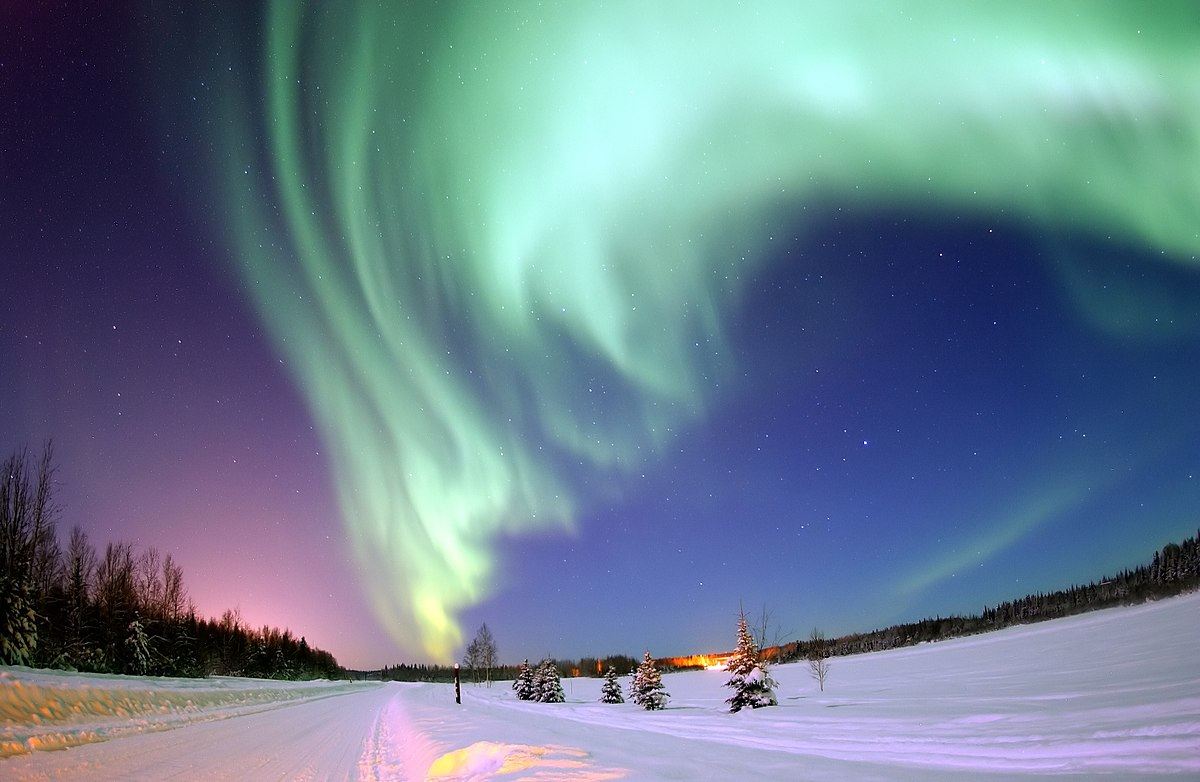
\includegraphics[width=70mm]{aurora1.jpg}  
\end{center}
\end{figure}

\subsection{使用手順}
まずは、ステンドガラス風にする処理に関して説明する。\\
プログラム実行時に第三引数として、ステンドグラスの細かさを指定するが、その値をコア数と呼ぶ。\\
以下、図5から図10は、コア数を徐々に大きくしていった結果である。粗いステンドグラス風の画像から細かくなるにつれて、入力画像に徐々に近づいていくのがわかる。
\begin{figure}[h]
    \begin{tabular}{cc}
          \begin{minipage}[t]{0.45\hsize}
        \centering
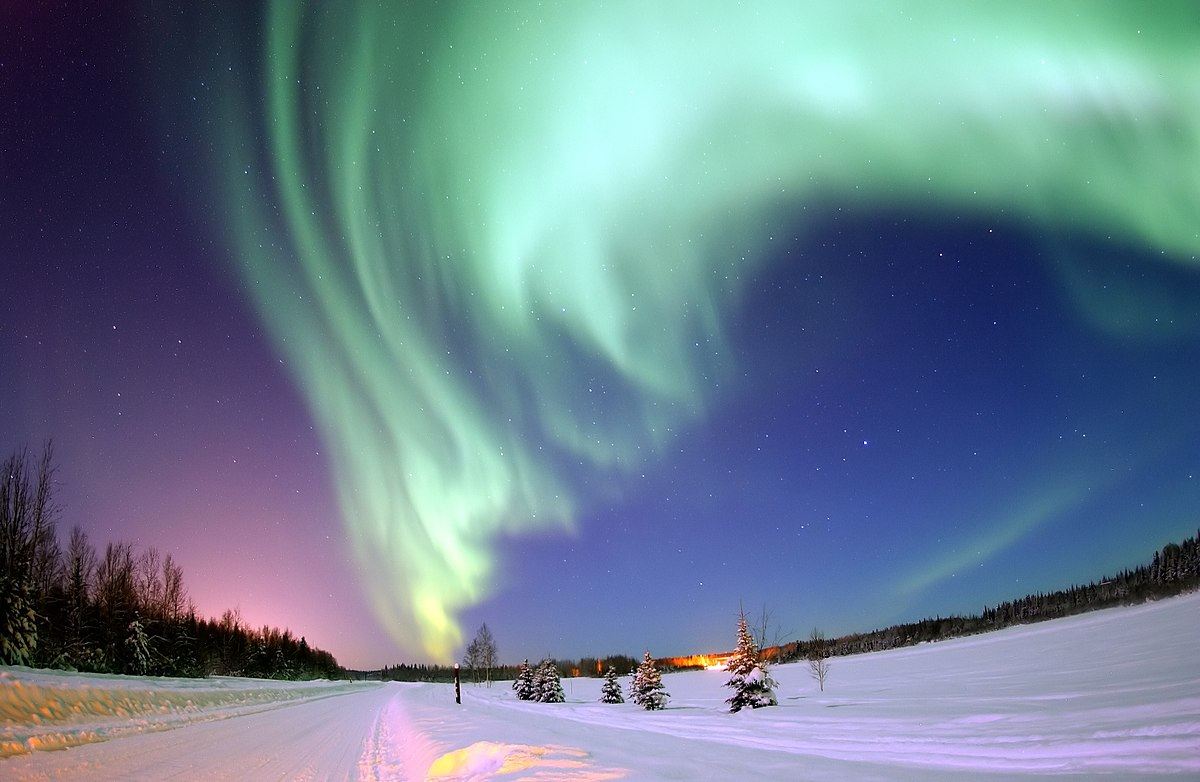
\includegraphics[keepaspectratio, width=66mm]{aurora1.jpg}  
 \caption{入力画像}
       \end{minipage} 
      
                \begin{minipage}[t]{0.45\hsize}
        \centering
\includegraphics[keepaspectratio,  width=66mm]{aurora200.jpg}  
 \caption{コア数=200}
 	\end{minipage}
	\\
 \begin{minipage}[t]{0.45\hsize}
        \centering	
\includegraphics[keepaspectratio,  width=66mm]{aurora500.jpg}
 \caption{コア数=500}
      \centering
 	\end{minipage}
	                \begin{minipage}[t]{0.45\hsize}
        \centering
\includegraphics[keepaspectratio,  width=66mm]{aurora1000.jpg}  
 \caption{コア数=1000}
      \centering
 	\end{minipage}
	   \end{tabular}
  \end{figure}
\newpage
\begin{figure}[h]
    \begin{tabular}{cc}
	                \begin{minipage}[t]{0.45\hsize}
        \centering
\includegraphics[keepaspectratio, width=66mm]{aurora5000.jpg}  
 \caption{コア数=5000}
      \centering
 	\end{minipage}
	
	                \begin{minipage}[t]{0.45\hsize}
        \centering
\includegraphics[keepaspectratio,  width=66mm]{aurora10000.jpg}  
 \caption{コア数=10000}
      \centering
 	\end{minipage}
    \end{tabular}
  \end{figure}
  
ステンドグラス風に画像を処理したあと、StainedMain.javaによって、取得した現在時刻を使い、時間帯によって画像の色味が変化するようにした。\\
ここでは、コア数50000でステンドグラス風画像処理を施したものを使用した。
\begin{figure}[h]
    \begin{tabular}{cc}
      %---- 最初の図 ---------------------------
      \begin{minipage}[t]{0.45\hsize}
        \centering
        \includegraphics[keepaspectratio, width=66mm]{aurora1-1.jpg}
        \caption{時刻が19:00-24:00または0:00-6:00の間}
    %    \label{ラベル1}
      \end{minipage} &
      \hspace{3mm}
      %---- 2番目の図 --------------------------
      \begin{minipage}[t]{0.45\hsize}
        \centering
        \includegraphics[keepaspectratio, width=66mm]{aurora1-2.jpg}
        \caption{時刻が6:00-16:00の間}
      %  \label{ラベル2}
      \end{minipage}
      %---- 図はここまで ----------------------
    \end{tabular}
  \end{figure} \\
  \begin{figure}[htbp]
\begin{center}
\includegraphics[width=66mm,height =45mm]{aurora1-3.jpg}   
\caption{時刻が16:00-19:00の間}
\end{center}
\end{figure}


\section{最後に}
今回最も凝ったのは、作品1の水面に反射している画像の作成でした。180度幾何回転させる段階までは順調に進んだのですが、左右反転させる処理が想像以上に難しく、座標を書いて試行錯誤を繰り返しました。普段、画像処理ソフトのボタン一押しで簡単に行なっているせいか、こんな簡単な処理がなぜ容易に実現できないのか、大変苦しく感じられました。クロマキー処理や背景との合成処理を行っているためか、複雑に考えさせられました。この経験のおかげで、普段使っているものの仕組みに興味が湧いたり、身の回りのソフトウェアの便利さに感謝の気持ちを持つきっかけとなりました。\\
\hspace{3mm}作品1では、ハワイと日没の地平線というお気に入りの画像を複数集めて、合成した、課題の趣旨に沿ったものを作成しました。しかし、どうしても今までの課題で行ってきた画像処理の枠を超えた画像処理を行いたく、一枚の画像のみを使用した作品2を作成しました。複数の画像を使っても良かったのですが、ステンドグラス風にしたかったため、画像処理の特性上、複数の画像を扱うメリットがなかったので一枚としました。\\
私は、ゲームの設定や、端末のデフォルトの壁紙などが時間帯によって変化していくのが、コンピュータ世界と現実の融合に感じられ、昔から好きでした。よって、作品2で時刻取得を組み込みました。自分でこのような挙動がプログラムできたのはとてもワクワクしました。\\
\hspace{3mm}画像処理に加えて、本説明書作成のために、LaTeXに挑戦できたことも大きな成長となりました。日本語出力を可能にするためのセットアップが大変だったり、コーディングのようなことをしながらWYSIWYGではないLaTeXを使って、画像の挿入位置を操作したりすることに慣れず、諦めかけたこともありました。しかし、今後論文の作成をすることなどを見越して、この経験は大変価値のあるものだったと考えています。
\section{おまけ}
\begin{figure}[h]
    \begin{tabular}{cc}
      %---- 最初の図 ---------------------------
      \begin{minipage}[t]{0.45\hsize}
        \centering
        \includegraphics[keepaspectratio, width=50mm]{ex2.jpg}
        \caption{理想形}
    %    \label{ラベル1}
      \end{minipage} &
      \hspace{3mm}
      %---- 2番目の図 --------------------------
      \begin{minipage}[t]{0.45\hsize}
        \centering
        \includegraphics[keepaspectratio, width=66mm]{copy_2.jpg}
        \caption{自作BGColor.java使用結果}
      %  \label{ラベル2}
      \end{minipage}
      %---- 図はここまで ----------------------
      \\
            \begin{minipage}[t]{0.45\hsize}
       \centering
      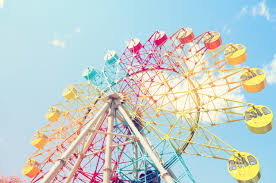
\includegraphics[width=50mm]{kanransya.jpg}
      \caption{図15の元画像}
            \end{minipage}

    \end{tabular}
  \end{figure} 
  この課題のコンセプトを固めるにあたって、様々な画像処理を見てきました。その中で、見慣れた配色や画像処理ではありましたが、いざ自力でやってみようとするとどのように実装していいのか、大変考えさせられるものが多々ありました。その一つが図14です。\\
  完成させられたらとても綺麗だろうと考え、挑戦してみたのですが、観覧車の中心が円形のようにピンクになっていることや、色の変化が縦横で共通しているものではなく、座標を使ってどのように色を調整していいのか分からず、自作ではなかなか実現できませんでした。\\
  しかし、パステルカラーで行う、と決めて色を研究して作ったフィルターがBGColor.javaというクラスなので、ここに記させていただきます。座標を使わずに実現する方法をこれから模索し、今後もチャレンジしてみたいと思います。

\end{document}